\documentclass{article}
\usepackage{hyperref}
\usepackage{listings}
\usepackage{color}
\usepackage{xcolor}
\usepackage{geometry}
\usepackage{graphicx}
\usepackage{amsmath}
\usepackage{caption}
\usepackage{subcaption}
\usepackage[capitalise]{cleveref}
\usepackage{wrapfig}
\usepackage{amssymb}

\geometry{margin=1in}
\pdfminorversion=6

\newcommand\TODO[1]{\textcolor{red}{TODO: #1}}

\newcommand\header[2]{
    \begin{center}
        {\large
        UCSD CSE 167 Assignment #1: \\
        \vspace{0.3cm}
        \Large
        #2}
    \end{center}
}

\definecolor{dkgreen}{rgb}{0,0.6,0}
\definecolor{gray}{rgb}{0.5,0.5,0.5}
\definecolor{mauve}{rgb}{0.58,0,0.82}
\lstset{frame=tb,
        aboveskip=3mm,
        belowskip=3mm,
        showstringspaces=false,
        columns=flexible,
        basicstyle={\small\ttfamily},
        numbers=none,
        numberstyle=\tiny\color{gray},
        keywordstyle=\color{blue},
        commentstyle=\color{dkgreen},
        stringstyle=\color{mauve},
        breaklines=true,
        breakatwhitespace=true,
        tabsize=2
}

% Taken from https://tex.stackexchange.com/questions/83085/how-to-improve-listings-display-of-json-files

\colorlet{punct}{red!60!black}
\definecolor{delim}{RGB}{20,105,176}
\colorlet{numb}{magenta!60!black}

\lstdefinelanguage{json}{
    basicstyle=\normalfont\ttfamily,
    numberstyle=\scriptsize,
    stepnumber=1,
    numbersep=8pt,
    showstringspaces=false,
    breaklines=true,
    frame=lines,
    tabsize=2,
    literate=
     *{0}{{{\color{numb}0}}}{1}
      {1}{{{\color{numb}1}}}{1}
      {2}{{{\color{numb}2}}}{1}
      {3}{{{\color{numb}3}}}{1}
      {4}{{{\color{numb}4}}}{1}
      {5}{{{\color{numb}5}}}{1}
      {6}{{{\color{numb}6}}}{1}
      {7}{{{\color{numb}7}}}{1}
      {8}{{{\color{numb}8}}}{1}
      {9}{{{\color{numb}9}}}{1}
      {:}{{{\color{punct}{:}}}}{1}
      {,}{{{\color{punct}{,}}}}{1}
      {\{}{{{\color{delim}{\{}}}}{1}
      {\}}{{{\color{delim}{\}}}}}{1}
      {[}{{{\color{delim}{[}}}}{1}
      {]}{{{\color{delim}{]}}}}{1},
}

\hypersetup{colorlinks=true}


\begin{document}

\header{2}{3D Software Rendering}

The previous homework focused on 2D graphics (which is already quite important!). In this homework, we're going 3D. We will define shapes in 3D, project them onto the screen, and render them. The projection is going to simulate how a camera (or our eyes) works. In particular, we will implement a \href{https://en.wikipedia.org/wiki/Pinhole_camera}{pinhole camera}. The light coming from an object goes through a very small hole and projects on a film (\cref{fig:pinhole}). 

\begin{figure}[h]
    \centering
    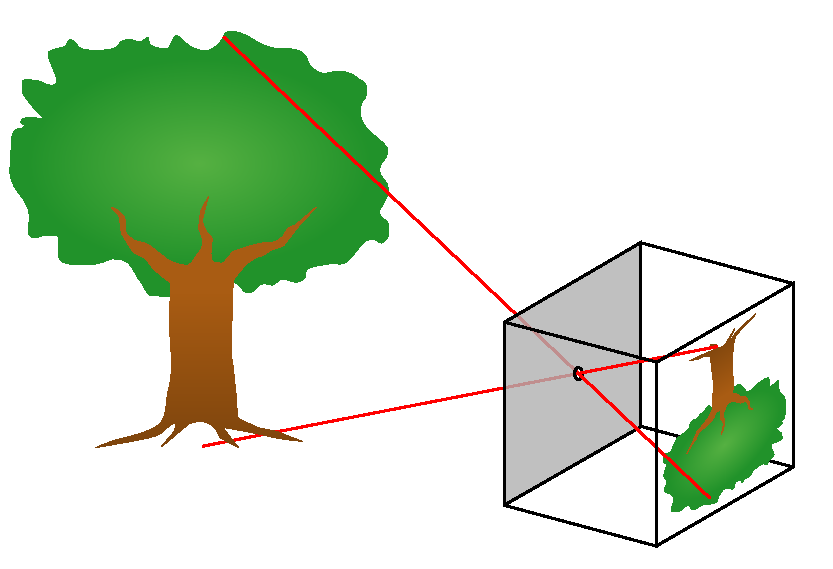
\includegraphics[width=0.5\linewidth]{imgs/pinhole.pdf}
    \caption{In this homework, we will implement 3D rendering by projecting 3D objects onto images. This is similar to a real-world camera. In particular, we will implement an ideal \href{https://en.wikipedia.org/wiki/Pinhole_camera}{pinhole camera}. Figure taken from \href{https://commons.wikimedia.org/wiki/File:Pinhole-camera.svg}{Wikipedia}.}
    \label{fig:pinhole}
\end{figure}

To facilitate the projection, we will focus on representing 3D surfaces, instead of the full volume. Instead of supporting multiple shapes (circles, squares, etc) like last time, we will focus on a single primitive: triangle. A main reason is that triangle has a very cool property: after perspective projection to 2D, it's still a triangle! (See \cref{fig:perspective}.) Many other shapes do not have this nice property -- a sphere projecting on to 2D can be an ellipse, a square projecting to the screen can become a general quadliteral.

\begin{figure}[h]
    \centering
    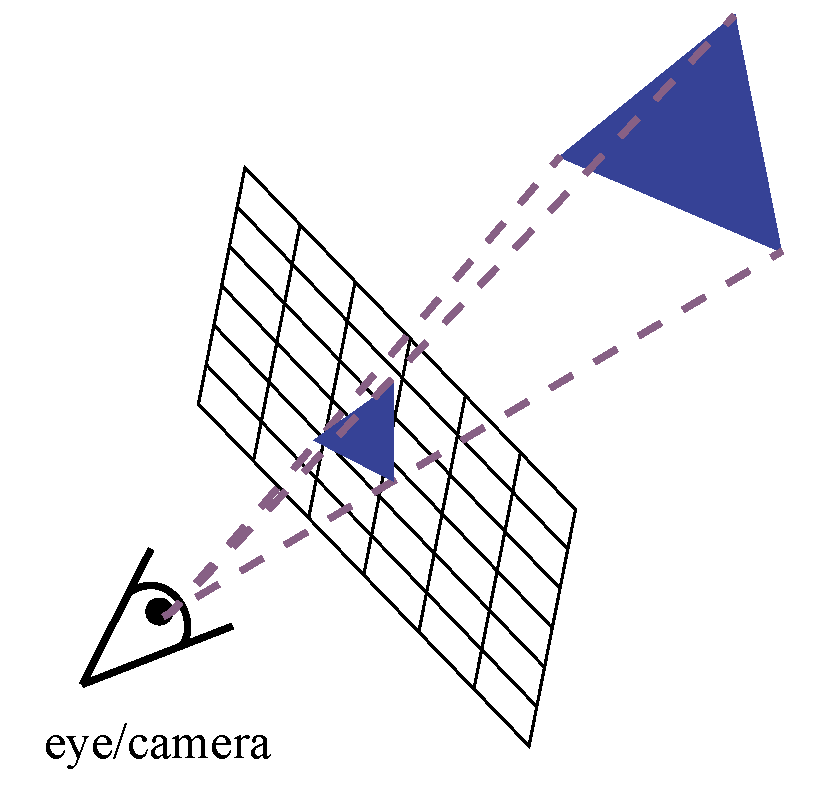
\includegraphics[width=0.5\linewidth]{imgs/perspective_projection.pdf}
    \caption{The perspective projection of a triangle.}
    \label{fig:perspective}
\end{figure}

\section{Rendering a single 3D triangle (20 pts)}
\label{sec:single_triangle}

Let's start simple and render just a single 3D triangle. Our plan is to first project the triangle to a 2D image plane, then we can directly use the code from our previous homework to render the projected triangle. Or even better, in the lectures we introduce a faster method using half-planes of the three edges of the triangle.

\begin{figure}[h]
    \centering
    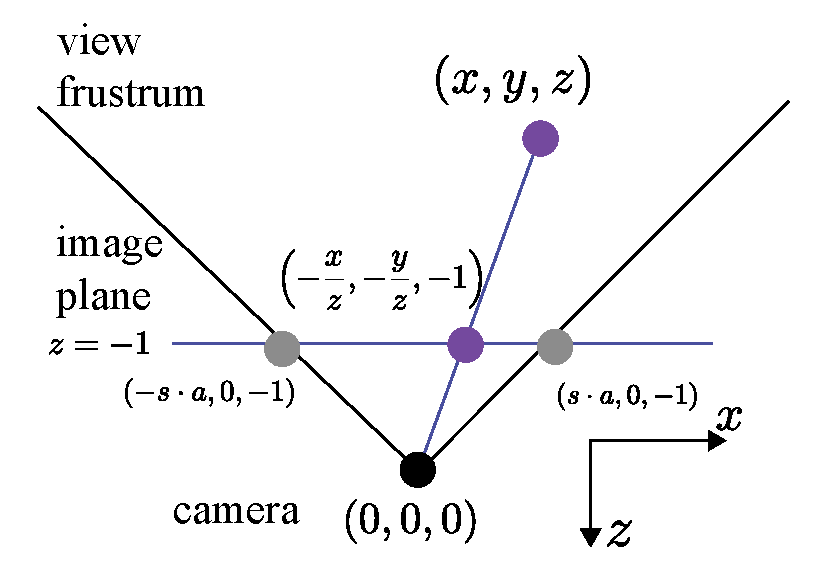
\includegraphics[width=0.5\linewidth]{imgs/perspective_transform.pdf}
    \caption{To perform perspective projection, we need to setup a coordinate system for the \emph{camera space}. The figure illustrates the configuration of the space (y is pointing outwards of the screen). The perspective projection of a point $(x, y, z)$ is then simply finding the intersection between the line formed by the point and the camera origin with the image plane. Since our image plane has a finite extent, we further clips all point outside of $[-sa, -s, -1] \times [sa, s, -1]$ where $a$ is the aspect ratio ($\frac{\text{image width}}{\text{image height}}$) and $s$ is the scaling factor controlling the size of our image. The clipping defines a \emph{view frustrum}.}
    \label{fig:perspective_transform}
\end{figure}

How do we project the triangle then? It's significantly easier if we assume a particular coordinate system of our camera. We will lift this assumption in the later part of the homework (by, you guess it, applying 3D transformations). 
\cref{fig:perspective_transform} illustrates the configuration and how to compute the projection by computing the intersection between the line formed by the point and the camera
origin with the image plane.

Furthermore, we need to define the extent of the image plane (we can't have an image with infinite size!). Note that our image can be a rectangle (instead of a square). We define the extent of the image plane to be $[-sa, -s, -1] \times [sa, s, -1]$: $s$ is a scaling factor that controls the size of the image (it's half of the sensor size), and $a$ is the aspect ratio ($\frac{\text{image width}}{\text{image height}}$). $s$ is related to the vertical \href{https://en.wikipedia.org/wiki/Field_of_view}{field of view} $\alpha$ of a camera:
\begin{equation}
s = \tan\left(\frac{\alpha}{2}\right).
\end{equation}
(A common bug in the previous years, when calculating the aspect ratio $a$, is that in C++, dividing two integers will round the results to an integer, e.g., $9/16=0$ in C++. Make sure you convert the types.)

Any point that lands outside of the extent of the image plane is discarded and not going to show up in our image. We call the set of points that are going to land on the image planes the \emph{view frustrum}. \cref{fig:perspective_transform} also visualizes the view frustrum.

Therefore, given a triangle with 3 vertices, we will project all three of them onto the image plane (\cref{fig:perspective_transform}). This generates a 2D triangle which we can then render using our previous homework's code.

\begin{figure}[h]
    \centering
    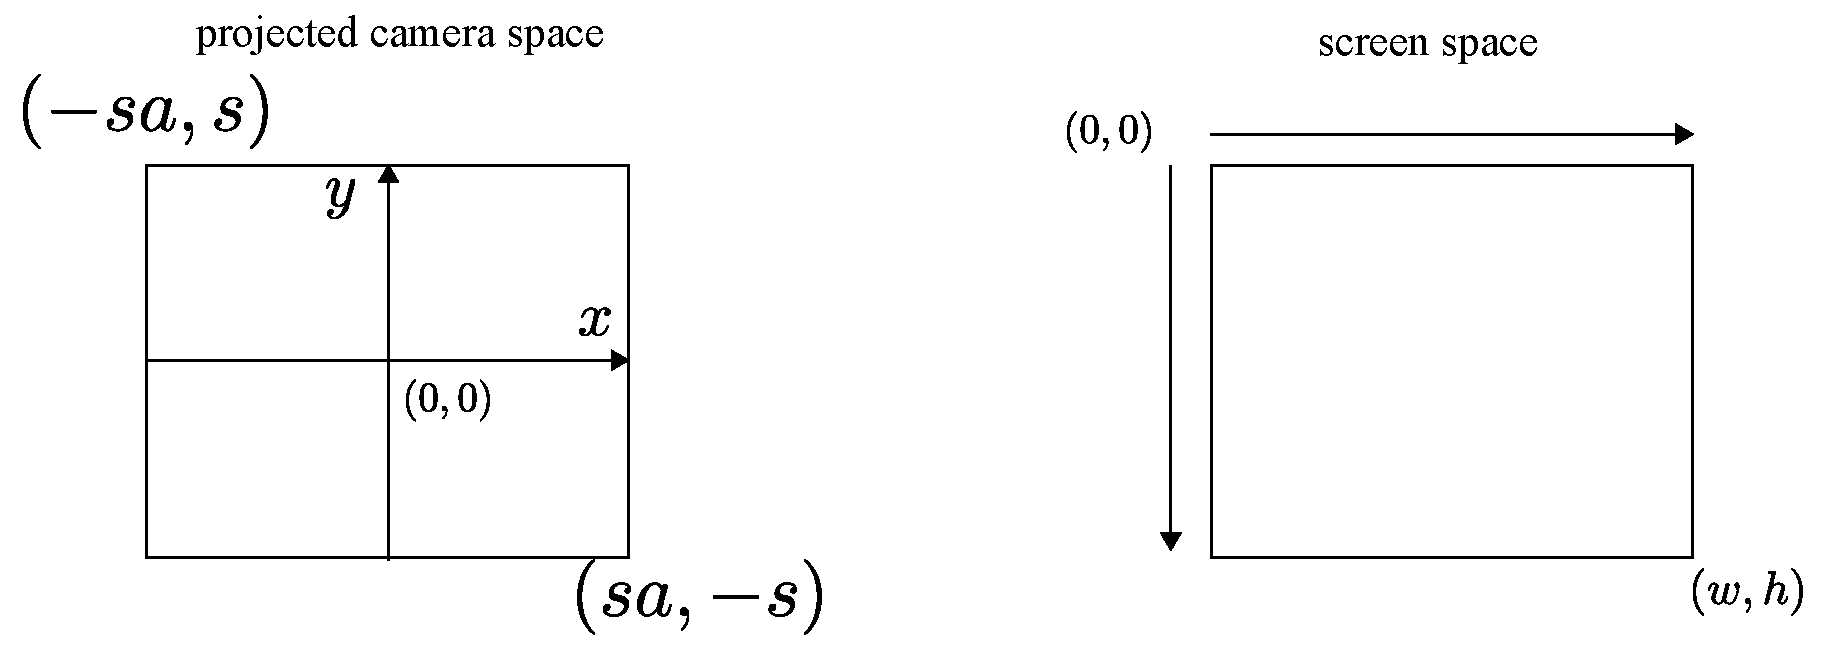
\includegraphics[width=0.9\linewidth]{imgs/camera_vs_screen.pdf}
    \caption{The different coordinate systems between our projected camera space and screen space.}
    \label{fig:camera_vs_screen}
\end{figure}

There are a few other complications though. Firstly, the projected point $(x', y', 1)$ is in the projected camera space after the projection. We will need to transform it into the screen space. Our screen space has $x$-axis pointing right with $y$-axis pointing down, and the extent is $[0, 0] \times [\text{width}, \text{height}]$. See \cref{fig:camera_vs_screen} (note that it is slightly different from the ``canvas space'' we used in Homework 1, where the $y$-axis pointed up). So we need to further convert the point $(x', y')$ from the projected camera space to screen space. Looking at \cref{fig:camera_vs_screen}, we can see that the we need to translate the origin, scale the axes, and flip the $y$ axis. We will give you the formula for the $x$-axis, and you should figure out the $y$-axis formula yourself:
\begin{equation}
x'' = w\frac{x'+sa}{2sa},
\label{eq:camera_to_screen}
\end{equation}
where $w$ is the width of the image.

The second complication is that a triangle vertex can be behind the camera i.e., $-z < 0$. In fact, even if $z$ is very close to zero, it can be still problematic: notice the division in \cref{fig:perspective_transform}. When $z$ is very close to zero, the division can be unstable due to limited floating point precision. 
Hence, we consider all points such that $-z < z_{\text{near}}$ to be behind the camera. 
$z_{\text{near}}$ is usually called the \emph{near clipping plane}.

Dealing with triangles with only one or two vertices behind the camera, and the other in front of the camera is a little bit tricky: we will need to implement \emph{clipping} (described below as a bonus). Instead, in this homework, we only require you only render the triangles where all three vertices are in front of the near plane. If even one of the vertices of a triangle is behind the near clipping plane, you should reject the triangle and not render it.

\begin{figure}[h]
    \centering
    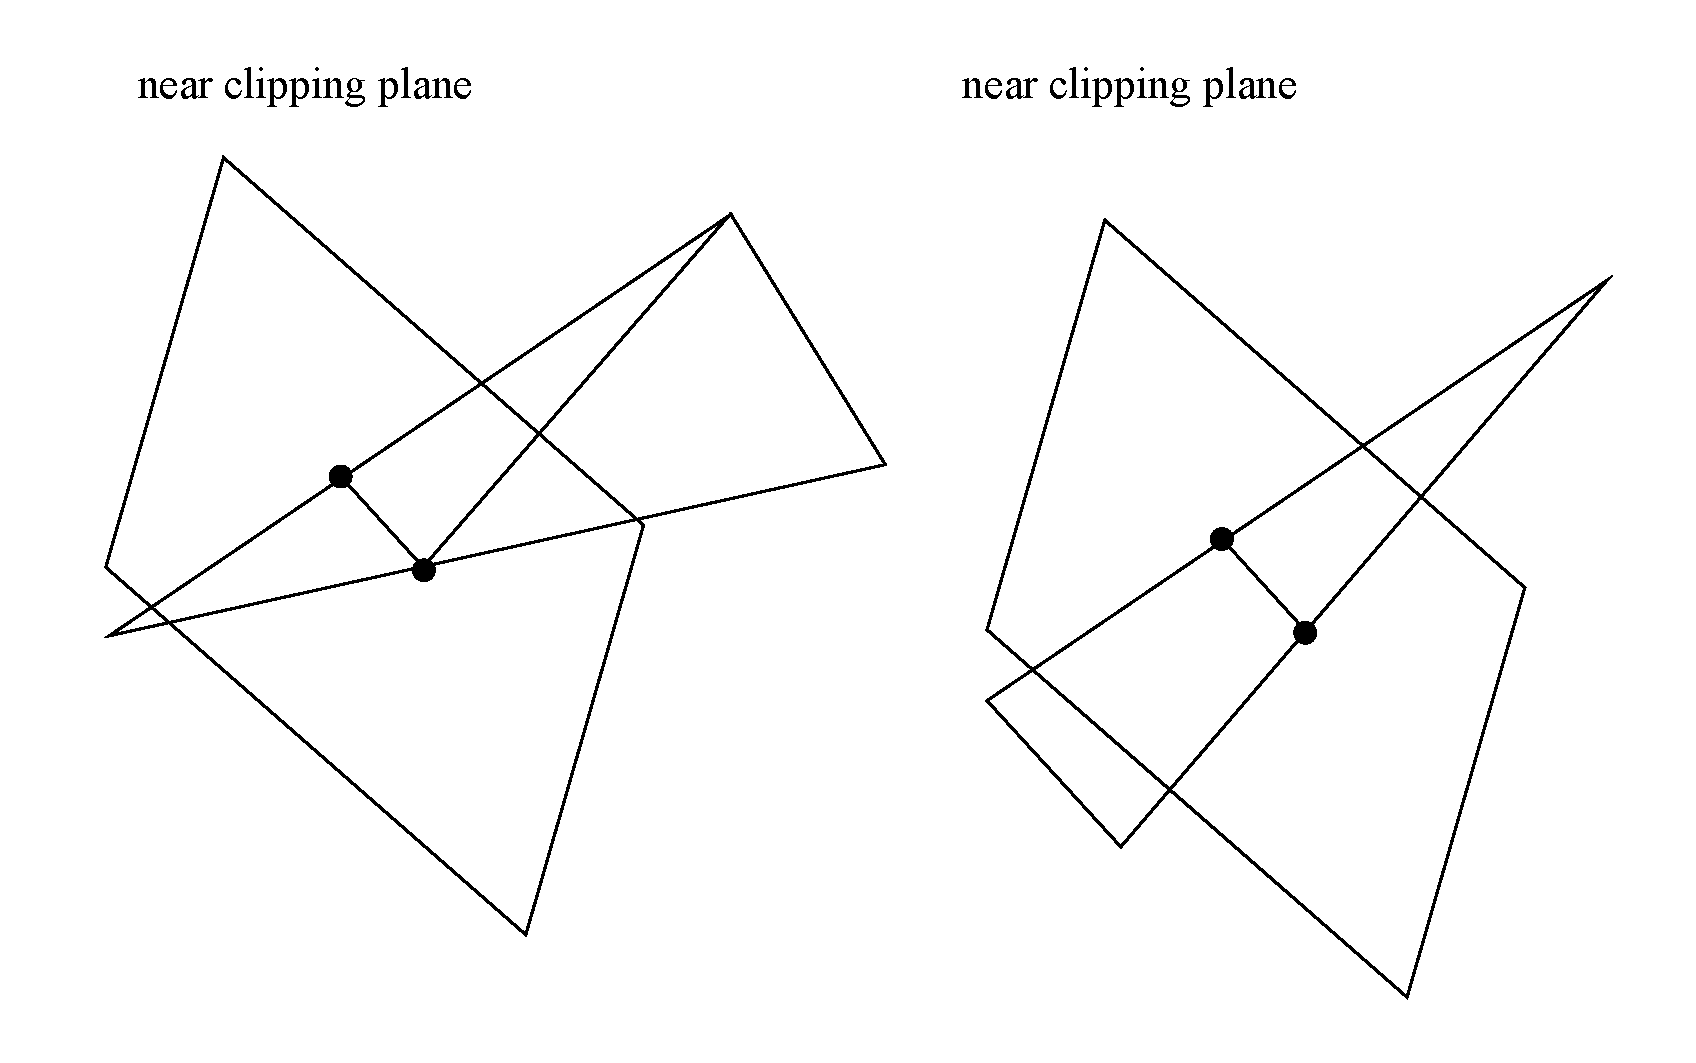
\includegraphics[width=0.7\linewidth]{imgs/triangle_clipping.pdf}
    \caption{If one or two vertices of a triangle is behind the near clipping plane, then (ideally) we would need to clip the triangle. If only one vertex is behind the clipping plane (left), then we need to clip and further split the resulting quadliteral into two triangles. If two vertices are behind the clipping plane (right), the clipped triangle is still a triangle.}
    \label{fig:triangle_clipping}
\end{figure}

We'll use the same antialiasing scheme we used in Homework 1, i.e., a $4\times4$ supersampling, for this entire homework. Make the background gray (0.5, 0.5, 0.5).

Implement your triangle rendering in \lstinline{hw_2_1()} in \lstinline{hw2.cpp}. To test your rendering, use the following commands:
\begin{lstlisting}[language=bash]
  ./balboa -hw 2_1 -s 1 -p0 -1 -1 -3 -p1 0 1 -3 -p2 1 -1 -3 -color 0.7 0.3 0.4 -znear 1e-6
  ./balboa -hw 2_1 -s 1 -p0 -1 0 -2 -p1 0 2 -4 -p2 1 -2 -5 -color 0.7 0.3 0.8 -znear 1e-6
  ./balboa -hw 2_1 -s 1 -p0 2 2 -1 -p1 -1 -1 -2 -p2 2 0 -3 -color 0.3 0.8 0.2 -znear 1e-6
  ./balboa -hw 2_1 -s 1 -p0 200 200 -100 -p1 1 3 -4 -p2 -2 -2 -2 -color 0.8 0.1 0.3 -znear 1e-6
\end{lstlisting}

We provide our rendering of the first command in \cref{fig:hw2_1}.
\begin{figure}[h]
    \centering
    
\includegraphics[width=0.5\linewidth]{imgs/hw_2_1.png}
    \caption{Reference rendering for homework 2.1.}
    \label{fig:hw2_1}
\end{figure}

In your submission, save the images generated by the second to fourth commands as
\begin{lstlisting}[language=bash]
outputs/hw_2_1_1.png
outputs/hw_2_1_2.png
outputs/hw_2_1_3.png
\end{lstlisting}
We'll compare your output with our rendering for grading.

\paragraph{Bonus: triangle clipping (10 pts).} In practice, instead of rejecting a triangle if one or two verices are behind the near clipping plane, graphics pipelines would implement triangle clipping (\cref{fig:triangle_clipping}). As a bonus, you will implement the clipping of the triangles and render them correctly even when some vertices are behind the near clipping plane. To speed up the computation, clipping is also often done with the entire 3D \href{https://en.wikipedia.org/wiki/Viewing_frustum}{view frustum}, discarding any triangles that are outside of the screen or too far away from the camera. We don't do it in this homework. 

\section{Rendering a triangle mesh (30 pts)}
\label{sec:triangle_mesh}

\begin{figure}[h]
    \centering
    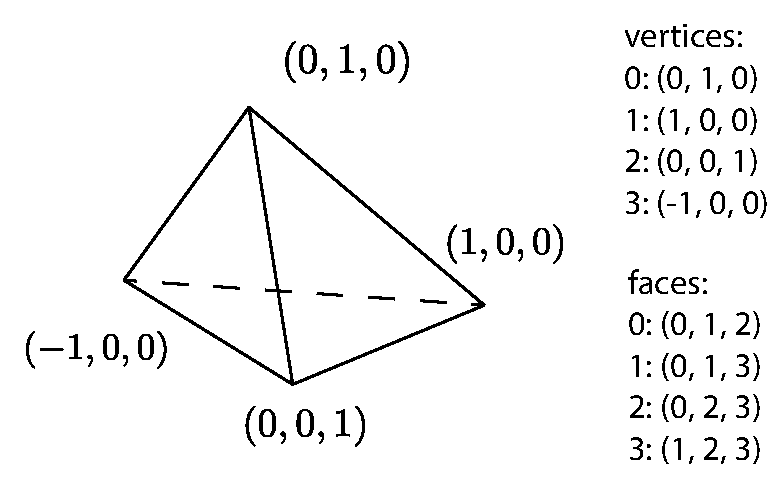
\includegraphics[width=0.7\linewidth]{imgs/triangle_mesh.pdf}
    \caption{A triangle mesh contains a list of vertices (3D positions) and a list of faces (3 integers pointing towards the index of the vertices). The figure shows a case of a triangle mesh with 4 vertices and 4 faces/triangles. The first face represents the triangle on the right side, the second face represents the triangle at the back, the third face represents the triangle on the left, and the last face represents the triangle at the bottom.}
    \label{fig:triangle_mesh}
\end{figure}

Next, we'll extend our previous code to handle more than one triangle. In computer graphics, we often store these triangles in a data structure called ``triangle mesh'' (\cref{fig:triangle_mesh}). Triangle mesh is a more efficient data structure than simply storing a list of triangles since many of the triangles would share vertices in graphics (really? when will it be better and when will it not be better?). To render triangle meshes, you need to go through the face array and loop through all the triangles. 

\begin{figure}[h]
    \centering
    
\includegraphics[width=0.4\linewidth]{imgs/cyclic.pdf}
    
\includegraphics[width=0.4\linewidth]{imgs/interpenetration.pdf}
    \caption{We cannot globally sort all objects into a single order by depth. The objects can form a cyclic order (left) or they can have interpenetration (right).}
    \label{fig:depth_order}
\end{figure}

An important difference, compared to the list of triangles we have in Homework 1, is to determine the depth order between all these triangles. That is, for a point inside a pixel, we need to decide which triangle is the one we actually see. The tricky part is, unlike Homework 1, it is impossible to globally sort the triangles to determine a depth order (\cref{fig:depth_order}).

Therefore, we need to know the depth value of all the triangles overlapping with the point in the pixel. That is, given a screen space point inside a projected triangle, we need to \emph{interpolate} from the depth values of the three vertices. This turns out to be slightly involved mathematically (code-wise it's actually not that much though, my implementation of the depth interpolation takes around 70 lines including lots of comments). 

To explain how to find the desired depth value, we need to explain what are \href{https://en.wikipedia.org/wiki/Barycentric_coordinate_system}{barycentric coordinates}. Any point $\mathbf{p}$ inside a triangle with three vertices $\mathbf{p}_0$, $\mathbf{p}_1$, $\mathbf{p}_2$ can be expressed using linear combination of the three vertices:
\begin{equation}
\mathbf{p} = b_0 \mathbf{p}_0 + b_1 \mathbf{p}_1 + b_2 \mathbf{p}_2,
\end{equation}
where $b_0 + b_1 + b_2 = 1$, $b_0 \geq 0$, $b_1 \geq 0$, and $b_2 \geq 0$. Given a point $\mathbf{p}$, we can compute the \textbf{unique} coefficients using \href{https://en.wikipedia.org/wiki/Cramer%27s_rule}{Cramer's rule}:
\begin{equation}
\begin{aligned}
b_0 &= \frac{\text{area}\left(\mathbf{p}, \mathbf{p}_1, \mathbf{p}_2\right)}{\text{area}\left(\mathbf{p}_0, \mathbf{p}_1, \mathbf{p}_2\right)} \\
b_1 &= \frac{\text{area}\left(\mathbf{p}_0, \mathbf{p}, \mathbf{p}_2\right)}{\text{area}\left(\mathbf{p}_0, \mathbf{p}_1, \mathbf{p}_2\right)} \\
b_2 &= \frac{\text{area}\left(\mathbf{p}_0, \mathbf{p}_1, \mathbf{p}\right)}{\text{area}\left(\mathbf{p}_0, \mathbf{p}_1, \mathbf{p}_2\right)}
\end{aligned}
\label{eq:barycentric_solve}
\end{equation}

To get the area of a triangle, you can use the length of the cross product between two of the edge vectors, which will give you the area of the parallelogram, you can then divide the parallelogram area by two. This works also for 2D triangles, you only need to pretend the 2D triangle is on a 3D plane (e.g., $z=0$).

\begin{figure}[h]
    \centering
    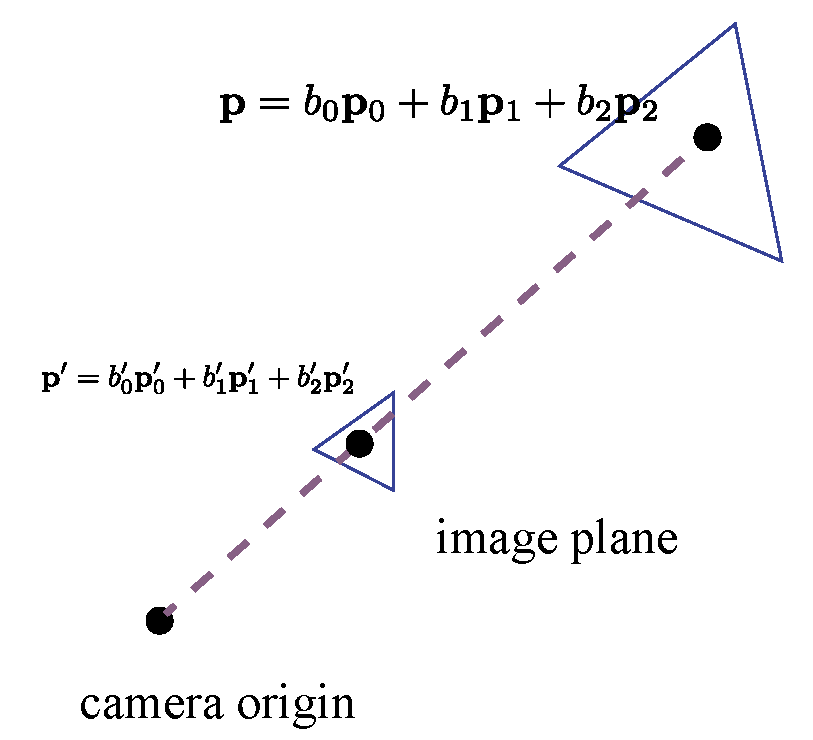
\includegraphics[width=0.5\linewidth]{imgs/perspective_interpolate.pdf}
    \caption{Given a point on image plane $p$', and a triangle with three vertices $\mathbf{p}_0$, $\mathbf{p}_1$, $\mathbf{p}_2$, we want to know the depth, i.e., the $z$ coordinate at the corresponding point $\mathbf{p}$.}
    \label{fig:perspective_interpolate}
\end{figure}

As illustrated in \cref{fig:perspective_interpolate}, our goal is, given an image plane point $\mathbf{p}'$ and a triangle with three vertices $\mathbf{p}_0$, $\mathbf{p}_1$, and $\mathbf{p}_2$, figure out the $z$ coordinate of the corresponding point $\mathbf{p}$. We want to use barycentric coordinates to help us. So we need to figure out what $b_0$, $b_1$, and $b_2$ are, so that we can interpolate the $z$ coordinates from $\mathbf{p}_0$, $\mathbf{p}_1$, and $\mathbf{p}_2$. Unfortunately, we cannot directly use \cref{eq:barycentric_solve}, since we don't know $\mathbf{p}$ (otherwise we would have known the answer already!). 

What we do know are the original vertices $\mathbf{p}_0$, $\mathbf{p}_1$, and $\mathbf{p}_2$, projected vertices $\mathbf{p}_0'$, $\mathbf{p}_1'$, and $\mathbf{p}_2'$, and our image plane point $\mathbf{p}'$. Furthermore, we know that $\mathbf{p}$ projects to $\mathbf{p}'$ and $\mathbf{p}_i$ projects to $\mathbf{p}_i'$. Given the projected vertices and the image plane point, we can compute the projected barycentric coordinates $b_0'$, $b_1'$, $b_2'$ using \cref{eq:barycentric_solve}. We want to relate the projected barycentric coordinates with the original ones.

Since $\mathbf{p}$ projects to $\mathbf{p}'$, we know that
\begin{equation}
\mathbf{p}' = \left(-\frac{\mathbf{p}.x}{\mathbf{p}.z}, -\frac{\mathbf{p}.y}{\mathbf{p}.z}, -1\right) 
= -\frac{\mathbf{p}}{\mathbf{p}.z}.
\end{equation}
(We use $\mathbf{p}.z$ to denote the z coordinate of point $\mathbf{p}$.)

Plugging in $\mathbf{p} = b_0 \mathbf{p}_0 + b_1 \mathbf{p}_1 + b_2 \mathbf{p}_2$ and $\mathbf{p}.z = b_0 \mathbf{p}_0.z + b_1 \mathbf{p}_1.z + b_2 \mathbf{p}_2.z$:
\begin{equation}
\mathbf{p}' = -\frac{b_0 \mathbf{p}_0 + b_1 \mathbf{p}_1 + b_2 \mathbf{p}_2}{b_0 \mathbf{p}_0.z + b_1 \mathbf{p}_1.z + b_2 \mathbf{p}_2.z}.
\end{equation}

Next, we know that $\mathbf{p}_0$ projects to $\mathbf{p}_0'$, $\mathbf{p}_1$ projects to $\mathbf{p}_1'$, and $\mathbf{p}_2$ projects to $\mathbf{p}_2'$:
\begin{equation}
\begin{aligned}
-\left(\mathbf{p}_0.z\right) \left(\mathbf{p}_0'\right) &= \mathbf{p}_0 \\
-\left(\mathbf{p}_1.z\right) \left(\mathbf{p}_1'\right) &= \mathbf{p}_1 \\
-\left(\mathbf{p}_2.z\right) \left(\mathbf{p}_2'\right) &= \mathbf{p}_2.
\end{aligned}
\end{equation}

Plugging in, we get
\begin{equation}
\mathbf{p}' = \frac{b_0 \left(\mathbf{p}_0.z\right) \mathbf{p}_0' + b_1 \left(\mathbf{p}_1.z\right) \mathbf{p}_1' + b_2 \left(\mathbf{p}_2.z\right) \mathbf{p}_2'}{b_0 \mathbf{p}_0.z + b_1 \mathbf{p}_1.z + b_2 \mathbf{p}_2.z}.
\end{equation}

Compare the above with:
\begin{equation}
\mathbf{p}' = b_0' \mathbf{p}_0' + b_1' \mathbf{p}_1' + b_2' \mathbf{p}_2',
\end{equation}
using the uniqueness of barycentric coordinates, we have:
\begin{equation}
\begin{aligned}
b_0' &= \frac{b_0 \mathbf{p}_0.z}{b_0 \mathbf{p}_0.z + b_1 \mathbf{p}_1.z + b_2 \mathbf{p}_2.z} \\
b_1' &= \frac{b_1 \mathbf{p}_1.z}{b_0 \mathbf{p}_0.z + b_1 \mathbf{p}_1.z + b_2 \mathbf{p}_2.z} \\
b_2' &= \frac{b_2 \mathbf{p}_2.z}{b_0 \mathbf{p}_0.z + b_1 \mathbf{p}_1.z + b_2 \mathbf{p}_2.z}.
\end{aligned}
\label{eq:projected_barycentric}
\end{equation}

We are almost there: we now want to express $b_0$, $b_1$, and $b_2$ using $b_0'$, $b_1'$, and $b_2'$. Let $B = b_0 \mathbf{p}_0.z + b_1 \mathbf{p}_1.z + b_2 \mathbf{p}_2.z$, we have:
\begin{equation}
\begin{aligned}
b_0 &= \frac{b_0' B}{\mathbf{p}_0.z} \\
b_1 &= \frac{b_1' B}{\mathbf{p}_1.z} \\
b_2 &= \frac{b_2' B}{\mathbf{p}_2.z}
\end{aligned}
\end{equation}

Furthermore, we know that $b_0 + b_1 + b_2 = 1$, so:
\begin{equation}
B = \frac{1}{\frac{b_0'}{\mathbf{p}_0.z} + \frac{b_1'}{\mathbf{p}_1.z} + \frac{b_2'}{\mathbf{p}_2.z}}.
\end{equation}

Rewriting \cref{eq:projected_barycentric} using the equation above, we have:
\begin{equation}
\begin{aligned}
\frac{\frac{b_0'}{\mathbf{p}_0.z}}{\frac{b_0'}{\mathbf{p}_0.z} + \frac{b_1'}{\mathbf{p}_1.z} + \frac{b_2'}{\mathbf{p}_2.z}} &= b_0 \\
\frac{\frac{b_1'}{\mathbf{p}_1.z}}{\frac{b_0'}{\mathbf{p}_0.z} + \frac{b_1'}{\mathbf{p}_1.z} + \frac{b_2'}{\mathbf{p}_2.z}} &= b_1 \\
\frac{\frac{b_2'}{\mathbf{p}_2.z}}{\frac{b_0'}{\mathbf{p}_0.z} + \frac{b_1'}{\mathbf{p}_1.z} + \frac{b_2'}{\mathbf{p}_2.z}} &= b_2
\end{aligned}.
\label{eq:inverse_depth_weighting}
\end{equation}
The equation above has an intuitive meaning: \textbf{the original barycentric coordinates can be obtained by the projected barycentric coordinate weighted by inverse depth}. We will use these equations again later in the homework.

Having the barycentric coordinates, we can finally get the desired depth:
\begin{equation}
\mathbf{p}.z = b_0 \mathbf{p}_0.z + b_1 \mathbf{p}_1.z + b_2 \mathbf{p}_2.z.
\label{eq:interpolated_depth}
\end{equation}

% To recap: given an image plane point and a triangle, we first convert it from screen space to camera space (using the inverse of \cref{eq:camera_to_screen}, recall \cref{fig:camera_vs_screen}). Then, we compute the projected barycentric coordinates $b_0'$, $b_1'$, and $b_2'$ using \cref{eq:barycentric_solve}. Using the projected barycentric coordinates and the depth at the three vertices, we convert them to the original barycentric coordinates using \cref{eq:inverse_depth_weighting}. Finally, we obtain the depth using \cref{eq:interpolated_depth} and use the depth to pick the triangle that is the closest to the pixel sample, but in front of the clipping plane.

To summarize, given an image plane point (e.g., pixel or subpixel center) and a triangle, we do the following:
\begin{enumerate}
    \item We first project triangle vertices to screen space, using the inverse of \cref{eq:camera_to_screen}, recall \cref{fig:camera_vs_screen}.
    \item If the image plane point is inside the triangle, we do the following:
    \item We convert the current image plane point from screen space to the projected camera space.
    \item We compute the projected barycentric coordinates $b_0'$, $b_1'$, and $b_2'$ using \cref{eq:barycentric_solve}.
    \item Using the projected barycentric coordinates and the depth at the three vertices, we convert them to the original barycentric coordinates using \cref{eq:inverse_depth_weighting}.
    \item Finally, we obtain the depth using \cref{eq:interpolated_depth} and use the depth to pick the triangle that is the closest to the pixel sample, but in front of the clipping plane.
\end{enumerate}

One final detail, in the lectures we discussed two variants for rendering multiple objects in a scene. For the \emph{ray tracing} style (i.e., for each pixel, check all triangles), you need to maintain the closest $z$ value when traversing all the triangles. For the \emph{rasterization} style (i.e., for each triangle, check all pixels), you need to maintain a whole image of $z$ values, and this is usually called the \emph{Z-buffer}. 
\begin{lstlisting}[language=Python]
# "Ray tracing style"
# For each pixel, check all triangles
for each pixel:
    for each antialiasing sample:
        z_min = infinity
        for each triangle:
            # check if the pixel center hits the triangle
            # overwrite color and z_min if the triangle is closer

# "Rasterization style"
# For each triangle, check all pixels
Z_buffer = Image(4 * w, 4 * h)
for each triangle:
    # project the triangle
    for each pixel:
        for each antialiasing sample:
            # check if the sample hits the triangle
            # overwrite color and Z_buffer[sample] if the triangle is closer
# Average the samples and downsize the image.
\end{lstlisting}
Notice how we handle the antialiasing in the rasterization method.
We will discuss the pros and cons of the two approaches in depth in the lectures.

Now you should be ready to implement the rendering of a triangle mesh! In this part, to specify the color of the triangles, in our triangle mesh, we further store a color per triangle. 

Our \lstinline{TriangleMesh} data structure looks like this:
\begin{lstlisting}[language=C++]
struct TriangleMesh {
    std::vector<Vector3> vertices; // 3D positions of the vertices
    std::vector<Vector3i> faces; // indices of the triangles
    std::vector<Vector3> face_colors; // per-face color of the mesh, only used in HW 2.2
    std::vector<Vector3> vertex_colors; // per-vertex color of the mesh, used in HW 2.3 and later
    Matrix4x4 model_matrix; // used in HW 2.4
};
\end{lstlisting}
\lstinline{faces} and \lstinline{face_colors} will always be the same length.

Go implement your triangle mesh rendering code in \lstinline{hw_2_2}. To test your implementation, use the command
\begin{lstlisting}[language=bash]
  ./balboa -hw 2_2 -s 1 -znear 1e-6 -scene_id 0
  ./balboa -hw 2_2 -s 1.5 -znear 1e-6 -scene_id 1
  ./balboa -hw 2_2 -s 0.4 -znear 1e-6 -scene_id 2
  ./balboa -hw 2_2 -s 0.5 -znear 1e-6 -scene_id 3
\end{lstlisting}
where \lstinline{[scene_id]} is the scene you want to render (0-3).

Our rendering for \lstinline{scene_id 0} is in \cref{fig:hw2_2}.
\begin{figure}[h]
    \centering
    
\includegraphics[width=0.5\linewidth]{imgs/hw_2_2.png}
    \caption{Reference rendering for homework 2.2.}
    \label{fig:hw2_2}
\end{figure}

In your submission, save your rendering of \lstinline{scene_id=1-3} as
\begin{lstlisting}[language=bash]
outputs/hw_2_2_1.png
outputs/hw_2_2_2.png
outputs/hw_2_2_3.png
\end{lstlisting}
We'll compare your output with our rendering for grading.

This part is more involved than the previous part. A way to debug is to render the same triangle as in \cref{sec:single_triangle} using your \cref{sec:triangle_mesh} code -- if they are different, then something is wrong and you can check what led to that problem. 

\section{Perspective-corrected interpolation (20 pts)}
\label{sec:interpolation}

So far, we have been rendering constant color triangles. It's time to make things more colorful. Instead of specifying \emph{face colors}, we'll specify \emph{vertex colors}, and interpolate them using barycentric coordinates.

It might be tempting to use the projected barycentric coordinates ($b_0', b_1'$ and $b_2'$) to interpolate the vertex colors, but this is incorrect: our triangle would be changing color based on the vertex depth if we do this (try it!). Instead, we want to interpolate using the original barycentric coordinates $b_0$, $b_1$, and $b_2$. Fortunately, we already know how to get them using \cref{eq:inverse_depth_weighting}! After computing the original barycentric coordinates, we'll just interpolate the vertex colors $C_0$, $C_1$, $C_2$ defined at the triangle vertices:
\begin{equation}
C = b_0 C_0 + b_1 C_1 + b_2 C_2.
\end{equation}
This is what people mean if they say they are doing \emph{perspective-corrected interpolation} in a renderer.

That's all you need to know to implement vertex color rendering! (I hope it's easier than the previous two.) Go and implement it in \lstinline{hw_2_3}. Test it using
\begin{lstlisting}[language=bash]
  ./balboa -hw 2_3 -s 1 -znear 1e-6 -scene_id 0
  ./balboa -hw 2_3 -s 1.5 -znear 1e-6 -scene_id 1
  ./balboa -hw 2_3 -s 0.4 -znear 1e-6 -scene_id 2
  ./balboa -hw 2_3 -s 0.5 -znear 1e-6 -scene_id 3
\end{lstlisting}

As usual, our rendering for \lstinline{scene_id 0} is in \cref{fig:hw2_3}.
\begin{figure}[h]
    \centering
    
\includegraphics[width=0.5\linewidth]{imgs/hw_2_3.png}
    \caption{Reference rendering for homework 2.3.}
    \label{fig:hw2_3}
\end{figure}

As usual, save your outputs for \lstinline{scene_id=1-3} as following.
\begin{lstlisting}[language=bash]
outputs/hw_2_3_1.png
outputs/hw_2_3_2.png
outputs/hw_2_3_3.png
\end{lstlisting}

\section{3D transformation (20 pts)}

So far we have assumed that everything is in the camera space and camera is always located at $(0, 0, 0)$ facing negative $z$ with up vector $y$. Let's add some transformations so that things are less restricted. Remember that in the 2D case in Homework 1, we use a $3 \times 3$ matrix to represent affine transformations. Here, we will use a $4 \times 4$ matrix. Like in 2D, we will support scaling, translation, and rotation (shearing is also possible, but we want to safe you some typing). Furthermore, we will support two kinds of new transformations: lookAt transform and perspective transform that we will talk about soon. The perspective transform implementation is optional, but implementing it might helpful understand parts of the next homework.

\begin{figure}[h]
    \centering
    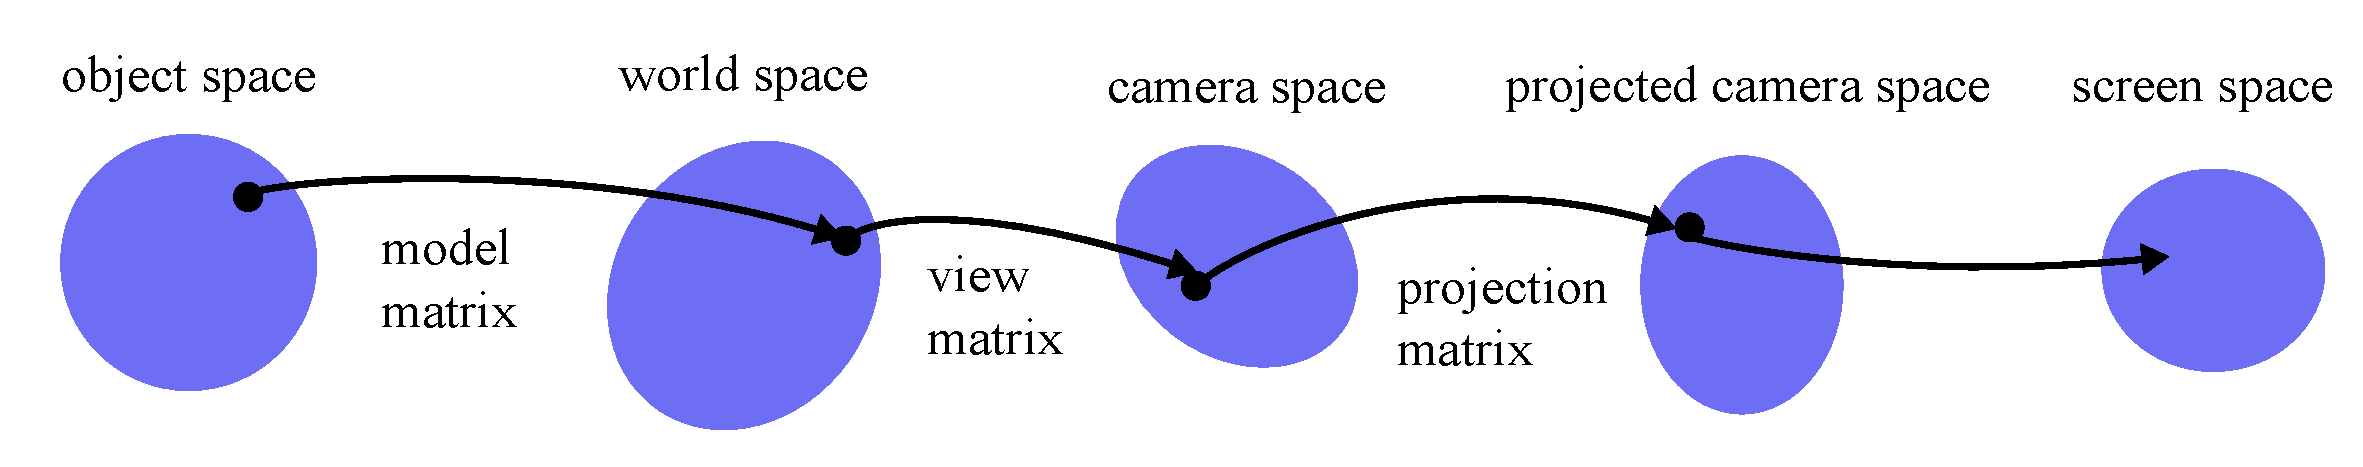
\includegraphics[width=0.8\linewidth]{imgs/3d_spaces.pdf}
    \caption{Spaces and the transformations between them in 3D.}
    \label{fig:3d_spaces}
\end{figure}

Before we explain the 3D transformations, we need to explain our spaces in 3D. Previously in 2D, we only had \emph{object space} and \emph{screen space}. The existence of the camera makes things slightly more complicated: the camera lives in the \emph{camera space} (the coordinate system in the previous parts), and the matrices now transform the objects into \emph{world space}. As a convention, we usually call the object-to-world transformation the \emph{model matrix} $M$, the world-to-camera transformation the \emph{view matrix} $V$, the camera-to-screen transformation the \emph{projection matrix} $P$ (yes, we can express the projection as a matrix! more on this later). Given a vertex $v$ on a 3D triangle mesh, we can chain the transformations to project it onto the screen space: $v'=PVMv$ (unfortunately, the combined matrix $PVM$ is usually called the ``MVP'' matrix). \cref{fig:3d_spaces} illustrates this. Note that the last two steps are what we did in \cref{sec:triangle_mesh}, where we project the triangles from camera space to projected camera space, and then to the screen space. 

\paragraph{Scaling and translation.} Scaling and translations are basically the same as in 2D:
\begin{equation}
\begin{bmatrix}
x' \\
y' \\
z' \\
1
\end{bmatrix}
=
\begin{bmatrix}
s_x & 0 & 0 & 0 \\
0 & s_y & 0 & 0 \\
0 & 0 & s_z & 0 \\
0 & 0 & 0 & 1
\end{bmatrix}
\begin{bmatrix}
x \\
y \\
z \\
1
\end{bmatrix}
\end{equation}

\begin{equation}
\begin{bmatrix}
x' \\
y' \\
z' \\
1
\end{bmatrix}
=
\begin{bmatrix}
1 & 0 & 0 & t_x \\
0 & 1 & 0 & t_y \\
0 & 0 & 1 & t_z \\
0 & 0 & 0 & 1
\end{bmatrix}
\begin{bmatrix}
x \\
y \\
z \\
1
\end{bmatrix}
\end{equation}

\paragraph{Rotation.} Rotation in 3D is a lot more complicated. Unlike 2D, which we pretty much only have two ways to rotate (clockwise or counterclockwise), in 3D there are infinitely many ways to rotate. We will talk about a lot of them in the lectures, but for this homework we will focus on rotating over a given axis $\mathbf{a}$ by $\theta$ degree. This is usually called an Axis/Angle representation of rotation. The following derivation is taken from the book \href{https://www.pbr-book.org/3ed-2018/Geometry_and_Transformations/Transformations}{Physically-based Rendering: From Theory to Implementation}, which is based on the famous \href{https://en.wikipedia.org/wiki/Rodrigues%27_rotation_formula}{Rodrigues' rotation formula}. Also see \href{https://thenumb.at/Exponential-Rotations/}{this excellent article} from Max Slater if you want to read more.

\begin{figure}[h]
    \centering
    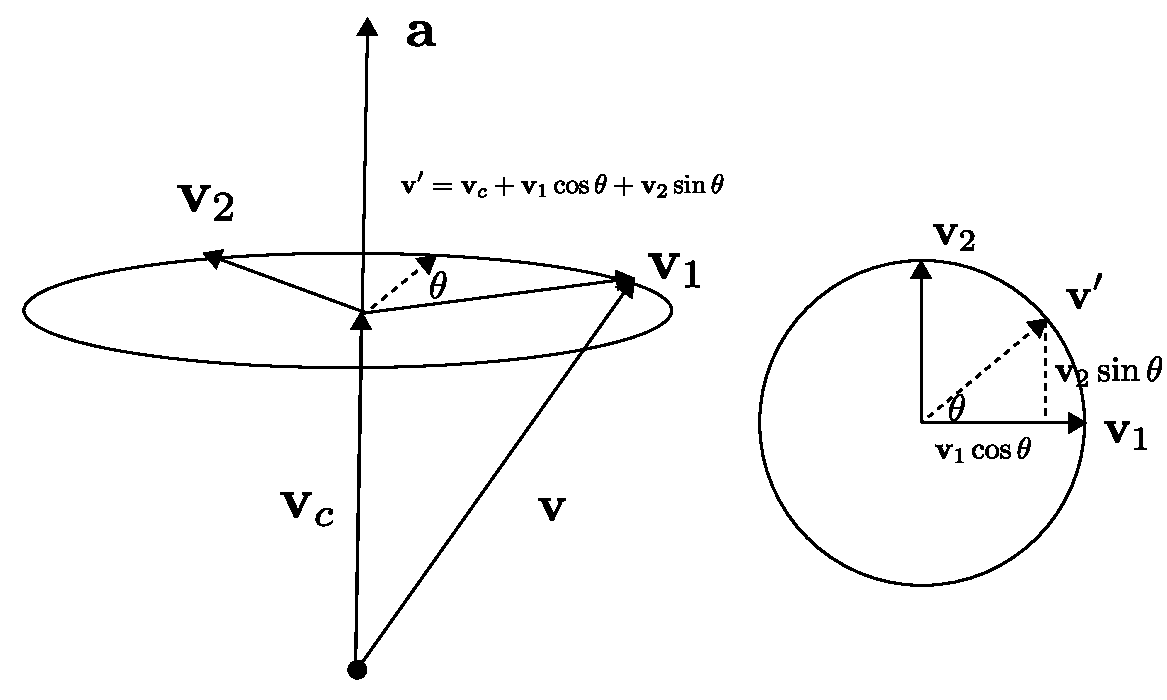
\includegraphics[width=0.5\linewidth]{imgs/rotate_axis.pdf}
    \caption{To rotate a vector $\mathbf{v}$ about an axis $\mathbf{a}$, we construct a plane with normal $\mathbf{a}$ with coordinate basis $\mathbf{v}_1$ and $\mathbf{v}_2$. The rotation can then be expressed as $\mathbf{v}' = \mathbf{v}_c + \cos\theta \mathbf{v}_1 + \sin\theta \mathbf{v}_2$.}
    \label{fig:rotate_axis}
\end{figure}

Our idea is to construct a coordinate system around the axis $\mathbf{a}$, then apply trigonometric identities in the 2D rotation plane. Instead of directly constructing the rotation matrix, it's easier to first derive what happens after we rotate a vector $\mathbf{v}$. \cref{fig:rotate_axis} illustrates the geometry: we first project the vector $\mathbf{v}$ to axis $\mathbf{a}$:
\begin{equation}
\mathbf{v}_c = \left(\mathbf{v} \cdot \mathbf{a}\right)\mathbf{a}.
\end{equation}
Next, we want to construct a coordinate system at $\mathbf{v}_c$. We choose the first axis to be:
\begin{equation}
\mathbf{v}_1 = \mathbf{v} - \mathbf{v}_c.
\end{equation}
The next axis $\mathbf{v}_2$ needs to be perpendicular to $\mathbf{v}_1$, so:
\begin{equation}
\mathbf{v}_2 = \mathbf{a} \times \mathbf{v}_1.
\end{equation}

With some trigonometry, we can then derive the rotated vector $\mathbf{v}'$:
\begin{equation}
\mathbf{v}' = \mathbf{v}_c + \cos\theta \mathbf{v}_1 + \sin\theta \mathbf{v}_2.
\end{equation}
(Note that our formulas are slightly different from the textbook above, since we use a right-handed coordinate system instead of a left-handed one.)

We can do a quick sanity test: let $\mathbf{a}$ be the $z$ axis. We have $\mathbf{v}_c = \left(0, 0, \mathbf{v}.z\right)$, $\mathbf{v}_1 = \left(\mathbf{v}.x, \mathbf{v}.y, 0\right)$, and $\mathbf{v}_2 = \left(-\mathbf{v}.y, \mathbf{v}.x, 0\right)$. Thus $\mathbf{v}' = \left(\cos\theta \mathbf{v}.x - \sin\theta \mathbf{v}.y, \cos\theta \mathbf{v}.x + \sin\theta \mathbf{v}.y, \mathbf{v}.z\right)$. We've recovered the standard 2D rotation.

To obtain the rotation matrix, we can plug in $\mathbf{v}=(1, 0, 0)$ to get the first column of the matrix, $\mathbf{v}=(0, 1, 0)$ to get the second column, and $\mathbf{v}=(0, 0, 1)$ to get the third column. Specifically, the first column of the $4\times4$ rotation matrix $R$ is given by:
\begin{equation}
\begin{bmatrix}
\mathbf{a}.x \mathbf{a}.x + (1 - \mathbf{a}.x \mathbf{a}.x) \cos\theta \\
\mathbf{a}.x \mathbf{a}.y (1 - \cos\theta) + \mathbf{a}.z \sin\theta \\
\mathbf{a}.x \mathbf{a}.z (1 - \cos\theta) - \mathbf{a}.y \sin\theta \\
0 
\end{bmatrix}.
\end{equation}
The second column is
\begin{equation}
\begin{bmatrix}
\mathbf{a}.y \mathbf{a}.x (1 - \cos\theta) - \mathbf{a}.z \sin\theta \\
\mathbf{a}.y \mathbf{a}.y + (1 - \mathbf{a}.y \mathbf{a}.y) \cos\theta \\
\mathbf{a}.y \mathbf{a}.z (1 - \cos\theta) + \mathbf{a}.x \sin\theta \\
0
\end{bmatrix}.
\end{equation}
The third column is
\begin{equation}
\begin{bmatrix}
\mathbf{a}.z \mathbf{a}.x (1 - \cos\theta) + \mathbf{a}.y \sin\theta \\
\mathbf{a}.z \mathbf{a}.y (1 - \cos\theta) - \mathbf{a}.x \sin\theta \\
\mathbf{a}.z \mathbf{a}.z + (1 - \mathbf{a}.z\mathbf{a}.z) \cos\theta \\
0
\end{bmatrix}.
\end{equation}

% To rotate about a given axis $\mathbf{u}$, our idea is to decompose it into a bunch of 2D rotations, so that $\mathbf{u}$ becomes the $z$ axis after transformation. We can then rotate about $z$ using a 2D rotation with the desired angle. We then need to invert other rotation to turn the given axis back to the original space. Precisely, we perform the 3D rotation in the following steps (also see \href{https://www.eng.uc.edu/~beaucag/Classes/Properties/OptionalProjects/CoordinateTransformationCode/Rotate%20about%20an%20arbitrary%20axis%20(3%20dimensions).html}{this article} from Paul Bourke):
% \begin{itemize}
%     \item rotate about the $x$ axis so that $\mathbf{u}$ lies in the $xz$ plane.
%     \item rotate about the $y$ axis so that $\mathbf{u}$ lies in the $z$ axis.
%     \item rotate about the $z$ axis by $\theta$ degree.
%     \item undo step (2).
%     \item undo step (1).
% \end{itemize}

% To rotate about $x$-axis by $\theta_x$ degree, we can easily extend the 2D rotation matrix:
% \begin{equation}
% R_x =
% \begin{bmatrix}
% 1 & 0 & 0 & 0 \\
% 0 & \cos \theta_x & -\sin \theta_x & 0 \\
% 0 & \sin \theta_x & \cos \theta_x & 0 \\
% 0 & 0 & 0 & 1
% \end{bmatrix}.
% \end{equation}

% How do we know how much to rotate about the $x$ axis, so that $\mathbf{u}$ lies in the $xz$ plane? There are more geometric ways to derive it, but I like to do it algebraically. We know that after the rotation, the $y$ component of the rotated vector should be $0$. Therefore, by directly applying the matrix vector product, we have:
% \begin{equation}
% \mathbf{u}.y \cos \theta_x - \mathbf{u}.z \sin \theta_x = 0.
% \end{equation}
% The equation above plus the trignometric identity $\cos^2\theta_x + \sin^2\theta_x = 1$ gives us a solution to $\theta_x$:
% \begin{equation}
% \begin{aligned}
% \cos \theta_x &= \frac{\mathbf{u}.z}{\sqrt{\mathbf{u}.y^2 + \mathbf{u}.z^2}} \\
% \sin \theta_x &= \frac{\mathbf{u}.y}{\sqrt{\mathbf{u}.y^2 + \mathbf{u}.z^2}} 
% \end{aligned}.
% \end{equation}

% We also need the inverse of the x rotation $R_x^{-1}$ for step (5) above.
% \begin{equation}
% R_x^{-1} =
% \begin{bmatrix}
% 1 & 0 & 0 & 0 \\
% 0 & \cos \theta_x & \sin \theta_x & 0 \\
% 0 & -\sin \theta_x & \cos \theta_x & 0 \\
% 0 & 0 & 0 & 1
% \end{bmatrix}.
% \end{equation}
% Here we use the identities $\cos -\theta_x = \cos \theta_x$ and $\sin -\theta_x = -\sin \theta_x$.

% After rotating by $R_x$, our axis becomes:
% \begin{equation}
% \mathbf{u}_x = \left(\mathbf{u}.x, 0, \sqrt{\mathbf{u}.y^2 + \mathbf{u}.z^2}\right).
% \end{equation}

% We next need to rotate about the $y$-axis by $\theta_y$ degree, so that $\mathbf{u}$ lies in the $z$ axis. The $y$-axis rotation matrix is:
% \begin{equation}
% R_y =
% \begin{bmatrix}
% \cos \theta_y & 0 & -\sin \theta_y & 0 \\
% 0 & 1 & 0 & 0 \\
% \sin \theta_y & 0 & \cos \theta_y & 0 \\
% 0 & 0 & 0 & 1
% \end{bmatrix}.
% \end{equation}

% We can use the same trick to determine $\theta_y$: after applying $R_y$ to $\mathbf{u}_x$, the $x$ component needs to be zero (and the $z$ component needs to be $1$):
% \begin{equation}
% \mathbf{u}.x \cos \theta_y - \sqrt{\mathbf{u}.y^2 + \mathbf{u}.z^2} \sin \theta_y = 0.
% \end{equation}
% Solving for $\theta_y$ (together with $\cos^2\theta_y + \sin^2\theta_y = 1$) we have
% \begin{equation}
% \begin{aligned}
% \cos \theta_y &= \sqrt{\mathbf{u}.y^2 + \mathbf{u}.z^2} \\
% \sin \theta_y &= \mathbf{u}.x.
% \end{aligned}
% \end{equation}

% The inverse $R_y^{-1}$ can be obtained similarly as $R_x^{-1}$.

% At this point, our rotation axis is the $z$ axis. We can rotate about the $z$ axis by the desired angle $\theta$:
% \begin{equation}
% R_z =
% \begin{bmatrix}
% \cos \theta & -\sin \theta & 0 & 0 \\
% \sin \theta & \cos \theta & 0 & 0 \\
% 0 & 0 & 1 & 0 \\
% 0 & 0 & 0 & 1
% \end{bmatrix}.
% \end{equation}

% Remember that we still need to invert the $x$ and $y$ rotations. Thus, our final rotation matrix is:
% \begin{equation}
% R = R_y^{-1} R_x^{-1} R_z R_y R_x.
% \end{equation}

% If you plug in the matrix values and actually multiply the matrices, you get the famous \href{https://en.wikipedia.org/wiki/Rodrigues%27_rotation_formula}{Rodrigues' rotation formula}.

\begin{figure}[h]
    \centering
    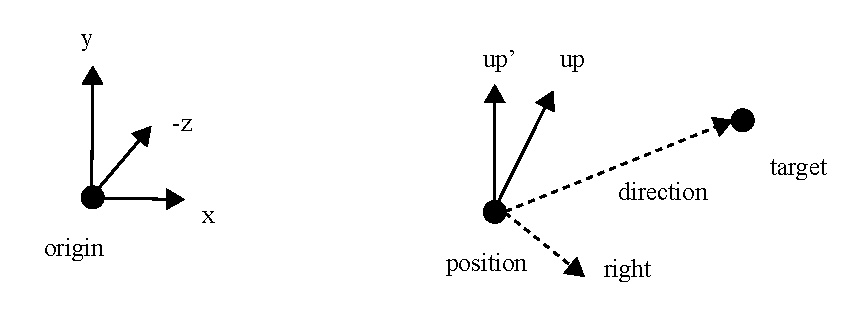
\includegraphics[width=0.7\linewidth]{imgs/lookat.pdf}
    \caption{The LookAt transform maps a coordinate frame based on the parameters \lstinline{position}, \lstinline{target}, and \lstinline{up}. $-z$ axis is mapped to the \lstinline{direction} of \lstinline{target - position}, $x$ axis is mapped to the cross product of \lstinline{direction} and \lstinline{up}, and $y$ axis is mapped to the cross product of \lstinline{right} and \lstinline{direction}.}
    \label{fig:lookat}
\end{figure}


\paragraph{LookAt.} The LookAt transform is useful for positioning cameras. The LookAt transform takes 2 3D points and a 3D vector as parameters: the \lstinline{position} of the object $\mathbf{p}$, the \lstinline{target} the object is looking at $\mathbf{t}$, and the \lstinline{up} vector $\mathbf{u}$ that describe the orientation of the object. \cref{fig:lookat} illustrates the geometry.

Given the input, we first compute where the camera should be facing using $\mathbf{p}$ and $\mathbf{t}$:
\begin{equation}
\mathbf{d} = \text{normalize}(t - p).
\end{equation} 
Given the \lstinline{direction} $\mathbf{d}$, we can then compute the \lstinline{right} vector $\mathbf{r}$ using cross product with the given \lstinline{up} vector $\mathbf{u}$:
\begin{equation}
\mathbf{r} = \text{normalize}\left(\mathbf{d} \times \mathbf{u}\right).
\end{equation}

We are not done yet though. Since the up vector $\mathbf{u}$ is not necessarily perpendicular to the camera direction $\mathbf{d}$, we do not have an orthonormal basis yet. Thus we recompute the up vector using the cross product between the right vector and the camera direction:
\begin{equation}
\mathbf{u}' = \mathbf{r} \times \mathbf{d}.
\end{equation}

Given these information, we can build our transformation matrix:
\begin{equation}
L = 
\begin{bmatrix}
\mathbf{r}.x & \mathbf{u}'.x & -\mathbf{d}.x & \mathbf{p}.x \\
\mathbf{r}.y & \mathbf{u}'.y & -\mathbf{d}.y & \mathbf{p}.y \\
\mathbf{r}.z & \mathbf{u}'.z & -\mathbf{d}.z & \mathbf{p}.z \\
0 & 0 & 0 & 1 
\end{bmatrix}
\end{equation}

The first column sends $x$ axis ($(1, 0, 0)$) to $\mathbf{r}$, the second column sends $y$ axis ($(0, 1, 0)$) to $\mathbf{u}'$, the third column sends $z$ axis to $\mathbf{d}$, and the last column translates the coordinate systems by $\mathbf{p}$.

Note that when applied to cameras, the matrix $L$ is designed to transform from camera space to world space. When constructing the view matrix (\cref{fig:3d_spaces}), we need to go from world space to the camera space. 

\paragraph{Perspective projection.}
Now we are at the coolest part. It turns out that with some math tricks, we can turn the perspective projection we did in the first part (\cref{fig:perspective_transform}) into a matrix multiplication as well! The trick is to introduce something called the \href{https://en.wikipedia.org/wiki/Homogeneous_coordinates}{homogeneous coordinates}. The idea is to make use of the 4th component of the vector. So far, we always assumed that the 4th component to be either $1$ or $0$ (when it's $0$, it's a vector instead of a point). From now on, our vectors can have arbitrary 4th component:
\begin{equation}
\begin{bmatrix}
x \\
y \\
z \\
w
\end{bmatrix}.
\end{equation}
The clever part is how we obtain the 3D vector from the 4D vector above: we define everything to be equivalent up to an arbitrary non-zero scaling:
\begin{equation}
\begin{bmatrix}
x \\
y \\
z \\
w
\end{bmatrix} =
\begin{bmatrix}
\frac{x}{w} \\
\frac{y}{w} \\
\frac{z}{w} \\
1
\end{bmatrix}.
\end{equation}

Following this definition, we can implement \cref{eq:projection} using the following matrix multiplication:
\begin{equation}
\begin{bmatrix}
x' \\
y' \\
z' \\
w'
\end{bmatrix} =
\begin{bmatrix}
1 & 0 & 0 & 0 \\
0 & 1 & 0 & 0 \\
0 & 0 & 0 & 1 \\
0 & 0 & -1 & 0
\end{bmatrix}
\begin{bmatrix}
x \\
y \\
z \\
1
\end{bmatrix}.
\end{equation}
Notice that
\begin{equation}
\begin{bmatrix}
x' \\
y' \\
z' \\
w'
\end{bmatrix}
=
\begin{bmatrix}
x \\
y \\
1 \\
-z
\end{bmatrix}
=
\begin{bmatrix}
-\frac{x}{z} \\
-\frac{y}{z} \\
-\frac{1}{z} \\
1
\end{bmatrix}.
\end{equation}
A bonus we get is that the new $z'$ component becomes the reciprocal of $-z$: we can directly use it for getting the barycentric coordinates (\cref{eq:inverse_depth_weighting})!

Remember that the projection above only projects within the camera space. We need to further convert to screen space (\cref{eq:camera_to_screen}). I'll let you figure out how the matrix should look like! 

Now you should have everything you need to complete this homework. 

Like Homework 1, we will describe the camera transformation and the meshes in a JSON scene file. 

A scene file would look like this:

\begin{lstlisting}[language=json]
{
    "camera":
    {
        "resolution": [640, 480],
        "transform": [
            {
                "lookat":
                {
                    "position": [0, 1, 0],
                    "target": [0, 0, -5],
                    "up": [0, 1, 0]
                }
            }
        ],
        "s": 1,
        "z_near": 1e-6
    },
    "background": [
        0.5, 0.5, 0.5
    ],
    "objects": [
        {
            "vertices": [
                -1.7,  1.0, -5.0,
                 1.0,  1.0, -5.0,
                -0.5, -1.0, -5.0,
                -2.5, -1.0, -5.0,
                -1.0,  1.5, -4.0,
                 0.2,  1.5, -4.0,
                 0.2, -1.5, -4.0
            ],
            "faces": [
                0, 1, 2,
                0, 2, 3,
                4, 5, 6  
            ],
            "vertex_colors": [
                0.75, 0.35, 0.35,
                0.35, 0.75, 0.35,
                0.35, 0.35, 0.75,
                0.75, 0.35, 0.75,
                0.35, 0.75, 0.75,
                0.75, 0.35, 0.75,
                0.75, 0.75, 0.35
            ],
            "transform": [
                {
                    "rotate": [45, 1, 1, 1]
                }
            ]
        }
    ]
}
\end{lstlisting}

Instead of directly specifying the vertices/faces in the JSON file, we can also use the \href{https://en.wikipedia.org/wiki/PLY_(file_format)}{Stanford PLY format}:
\begin{lstlisting}[language=json]
{
    "camera":
    {
        "resolution": [640, 480],
        "transform": [
            {
                "lookat":
                {
                    "position": [1, 1, 0],
                    "target": [0, 0, -5],
                    "up": [0, 1, 0]
                }
            }
        ],
        "s": 1,
        "z_near": 1e-6
    },
    "background": [
        0.5, 0.5, 0.5
    ],
    "objects": [
        {
            "filename": "tetrahedron.ply",
            "transform": [
                {"scale": [1.5, 0.8, 0.7]},
                {"translate": [0.5, -0.3, 0.2]}
            ]
        }
    ]
}
\end{lstlisting}
The PLY file is human readable (when in the ``ascii'' mode) and looks like this:
\begin{lstlisting}
ply
format ascii 1.0
comment Created by Blender 3.4.1 - www.blender.org
element vertex 4
property float x
property float y
property float z
property float red
property float green
property float blue
element face 4
property list uchar uint vertex_indices
end_header
-0.483444 0.826069 -2.307457 0.75 0.35 0.35
1.152029 -1.111880 -1.928058 0.35 0.75 0.35
1.485437 0.880605 -2.239198 0.35 0.35 0.75
0.594299 0.143237 -1.466344 0.75 0.35 0.75
3 0 1 2
3 1 3 2
3 3 1 0
3 2 3 0
\end{lstlisting}

The scene will be parsed into the following scene data structure:
\begin{lstlisting}[language=C++]
struct Camera {
    Matrix4x4 cam_to_world;
    Vector2i resolution;
    Real s;
    Real z_near;
};

struct Scene {
    Camera camera;
    Vector3 background;
    std::vector<TriangleMesh> meshes;
};
\end{lstlisting}

Like in Homework 1, your first task is to implement the transformations in \lstinline{parse_transformation} in \lstinline{hw2_scenes.cpp}. Next, you'll render the parsed scene in \lstinline{hw_2_4} in \lstinline{hw2.cpp}.

\textbf{Important}: the \lstinline{transform} in the camera describes the transformation from camera to world, and that's what we store in \lstinline{Camera::cam_to_world}. The ``view matrix'' in \cref{fig:3d_spaces} is the inverse of \lstinline{cam_to_world}.

To test your rendering, use the following commands:
\begin{lstlisting}[language=bash]
  ./balboa -hw 2_4 ../scenes/hw2/two_shapes.json
  ./balboa -hw 2_4 ../scenes/hw2/tetrahedron.json
  ./balboa -hw 2_4 ../scenes/hw2/cube.json
  ./balboa -hw 2_4 ../scenes/hw2/prism.json
  ./balboa -hw 2_4 ../scenes/hw2/teapot.json
\end{lstlisting}

Our renderings of the \lstinline{two_shapes} and \lstinline{tetrahedron} scenes are shown in \cref{fig:hw2_4}.
\begin{figure}[h]
    \centering
    
\includegraphics[width=0.49\linewidth]{imgs/hw_2_4_two_shapes.png}
    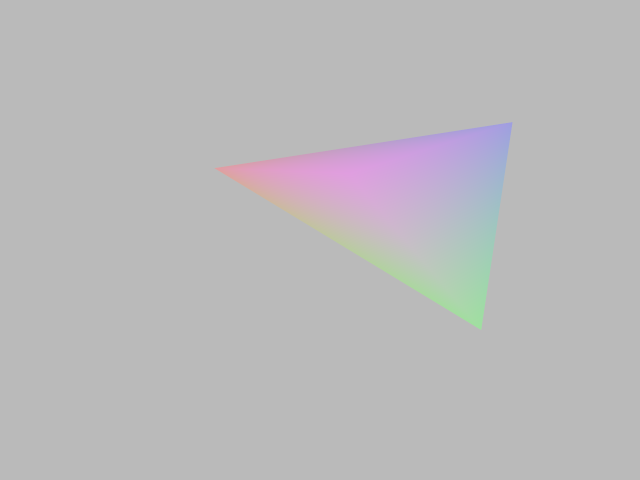
\includegraphics[width=0.49\linewidth]{imgs/hw_2_4_tetrahedron.png}
    \caption{Reference renderings for homework 2.4.}
    \label{fig:hw2_4}
\end{figure}

Save your outputs for the scenes above as following.
\begin{lstlisting}[language=bash]
outputs/hw_2_4_cube.png
outputs/hw_2_4_prism.png
outputs/hw_2_4_teapot.png
\end{lstlisting}

Note that the last teapot scene contains 1570 triangles, so it might take a bit of time to render it (it took 30 seconds in my implementation). By the way, the teapot is the famous \href{https://en.wikipedia.org/wiki/Utah_teapot}{Utah teapot} made by Martin Newell when doing his Ph.D. at Utah in the early days of computer graphics.

\section{Design your own scenes (10 pts)}

As usual, design a scene yourself and submit the scene and your rendering to us. We will give extra credits to people who impress us. Feel free to download 3D model files on the internet (please credit the authors and let us know where you downloaded it). Note that our parser assumes existence of the following attributes in a vertex: x, y, z, r, g, b, so if your downloaded model does not have the RGB information stored in the vertices, it may not parse correctly. Our parser also assumes that the model is a triangle mesh -- some meshes have general polygons and need to be triangulated before importing to balboa.

\section{Bonus: animation (15 pts)}
Like Homework 1, generate an animation by interpolating between transformations. To interpolate between rotations, read the \href{https://thenumb.at/Exponential-Rotations/}{article} from Max Slater. You will only get the full 15 points if you have interpolated rotation.
Feel free to modify any part of the code in balboa. You can use \href{https://trac.ffmpeg.org/wiki/Slideshow}{ffmpeg} to convert a sequence of images into a video file.

\section{Bonus: ray casting (20 pts)}
Follow \href{https://raytracing.github.io/books/RayTracingInOneWeekend.html}{ray tracing in one weekend} and implement a ray caster that renders our JSON scenes. For coloring, use the 3D barycentric coordinates to interpolate the vertex color as in \cref{sec:interpolation}. 
For ray-triangle intersection, you can use the \href{https://en.wikipedia.org/wiki/M%C3%B6ller%E2%80%93Trumbore_intersection_algorithm}{Möller–Trumbore intersection algorithm}, which will give you the barycentric coordinates of the triangle along with the intersection (feel free to copy paste code for this part). 
You will find that a ray caster is actually easier to implement than our projection-based rasterizer, but we want you to know different ways to render and the rasterizer is how the most of the current GPU works except for ray tracing hardware.

\section{Bonus: occlusion culling (20 pts)} 

During rasterization-style rendering, if we can prove that a triangle is completely blocked by some other triangles (using the current Z buffer), we can completely skip the rendering of the triangle to speed up our rendering. 
This is called \href{https://en.wikipedia.org/wiki/Z-buffering#Z-culling}{occlusion culling} or Z-culling. 
Read the paper \href{https://dl.acm.org/doi/10.1145/166117.166147}{Hierarchical Z-Buffer Visibility} from Greene et al. and implement occlusion culling using a hierarchical Z buffer. 
Our test scenes do not have heavy occlusion, so you will need to design your own scenes to show the speedup.

%\bibliographystyle{plain}
%\bibliography{refs}

\end{document}
